\documentclass[a4paper]{article}

\usepackage[margin=2.5cm,headheight=50pt,includeheadfoot]{geometry}

\usepackage{amsfonts}
\usepackage{amsmath}
\usepackage{graphicx}
\usepackage{fancyhdr}
\pagestyle{fancy}
\renewcommand{\headrulewidth}{2pt}

\usepackage{xcolor}

\rhead{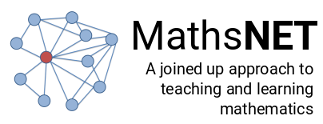
\includegraphics[width=5cm]{../../html/assets/img/logo.png}}
\lhead{\Huge SOR3012: Tutorial week 6}

\begin{document}

\section{Aim}

The aim of the tutorial this week is to look at the final project for the central limit theorem section in order to determine how to attack this problem.

\section{Bring}

Please bring all your notes for this module as well as appropriate items of stationery.

\section{Approach}

You will start by working on your own and I will then put you into groups of two or three after you have had a chance to think about the problem by yourself.    Remember the problem in question is 
the following:

\begin{quotation}
The Mandelbrot set contains all the complex numbers, $c$, for which the orbit of 0 under iteration of the quadratic map: $z_{n+1} = z_n^2 + c$ remains bounded.  You have been give a python script that 
gives a method for calculating the area of the Mandelbrot set and you have been asked to discuss how the code work and how the code can be extended so that also can get confidence limits on the 
estimate of the area that is generated.
\end{quotation}

Here are some suggestions that you might want to use in order to determine the solution to this problem:

\begin{enumerate}
 \item Are there words in the statement of the problem that you do not understand?  What are those words?  Perhaps you can highlight the words that you don't understand on this handout so that you can 
discuss them when you are put into groups?  Where might you look those words up?  Do you understand the definitions of the words now that you have found them?

 \item What problems that are similar to this one have you seen as you worked through the apply and extend sections during the last three weeks?
 
 \item Do you understand every line of the computer program that you have been given?  Could you for instance copy the code and write a comment that describes what is being calculated on each line?  
Are there lines you don't understand?  If there are lines you don't understand this is something that you can discuss when you are put into groups.  

 \item Do you understand how the information in the statement of the problem has been translated into python code?  As a case in point, the statement of the problem contains a formula.  Where is that 
formula in the python code?  Is the formula the only mathematical information that is contained in the statement of the problem? 
 
 \item What is the formula for calculating confidence limits?  Do you know how to obtain all the quantities that need to be inserted into this formula?  
\end{enumerate}




\end{document}
